\documentclass{beamer}

\usetheme{default}
\usecolortheme{rose}
\usepackage{hyperref}
\newcommand{\ignore}[1]{}
\setbeamerfont{alerted text}{series=\itshape}
\addtobeamertemplate{navigation symbols}{}{%
    \usebeamerfont{footline}%
    \usebeamercolor[fg]{footline}%
    \hspace{1em}%
    \insertframenumber/\inserttotalframenumber
}

\newcommand{\pr}{\mathbb{P}}

\title{Conditional Probability and Counting Rules}

% A subtitle is optional and this may be deleted
\subtitle{STAT-UB.0001 Statistics for Business Control}

\author{Ningshan Zhang}
% - Give the names in the same order as the appear in the paper.
% - Use the \inst{?} command only if the authors have different
%   affiliation.

\institute[New York University] % (optional, but mostly needed)
{
  IOMS Department\\
  nzhang@stern.nyu.edu
}
\date{Jul 10, 2018}



% Let's get started
\begin{document}

%-------------------
\begin{frame}
  \titlepage
\end{frame}



%\section{Conditional Probability}
% Section and subsections will appear in the presentation overview
% and table of contents.
\begin{frame}{Review}
\begin{itemize}
\item Random experiment, sample point, sample space
\item Probability
\item Events, union and intersection, mutually exclusive events, complementary event
\item Additive rule
\item Conditional probability, multiplicative rule
\end{itemize}
\end{frame}


\begin{frame}{Statistical Independence}
A and B are independent events if the occurrence of A doesn’t change the probability that B occurs. Formally,
\begin{itemize}
    \item $\pr(A \cap B)=\pr(A)\pr(B)$
    \item Equivalently, $\pr(A \mid B)=\pr(A)$
    \item Equivalently, $\pr(B \mid A)=\pr(B)$
\end{itemize}

\vspace{\stretch{0.5}}
Example:
\begin{itemize}
    \item Are mutually exclusive events independent?
    \item Flip two coins, A =``the first coin shows Heads'', B = ``The second coin shows Heads''.
\end{itemize}

\end{frame}

\begin{frame}{Statistical Independence}
Statistical independence simplifies calculation of probabilities:
$$\pr(A\cap B) =\pr(A)\pr(B).$$

\vspace{\stretch{0.5}}
Example: Suppose that you flip two fair coins. Let A =``the first coin shows Heads'', 
B = ``The second coin shows Heads''. Find the probability of getting Heads on both coins, i.e.\ find 
$\pr(A \cap B)$.
\end{frame}

\begin{frame}{Bayes' Rule}
    A tool to relate $\pr(A\mid B)$ to $\pr(B | A)$:
    $$ \pr(B\mid A) = \frac{\pr(A\mid B) \pr(B)}{\pr(A)}$$%, \quad \pr(A\mid B) = \frac{\pr(B\mid A) \pr(A)}{\pr(B)}$$ 

\vspace{\stretch{0.5}}
Example: With probability 0.15, a person will pass the job interview for a Data Analyst position. 
Among those who passed the interview, 60\% had taken college courses in Statistics. It
happens also that 30\% of all those who interviewed had college courses in
Statistics. Find the probability that a person with college courses in Statistics
will pass the job interview.
\end{frame}

\begin{frame}{Bayes' Rule}
    More generally, given $k$ mutually exclusive events $B_1,B_2,\dots,B_k$ such that $\pr(B_1) + \pr(B_2) + \dots + \pr(B_k)=1$, then
    \begin{align*}
        \pr(B_i \mid A) & = \frac{\pr(A \cap  B_i) }{\pr(A)}\\
                        & =
        \frac{\pr(A\mid B_i) \pr(B_i)}
        {\pr(A\mid B_1)\pr(B_1) + \dots + \pr(A\mid B_k) \pr(B_k)}
    \end{align*}

\vspace{\stretch{0.5}}
    Example: Suppose that 1\% of population have a special disease. A blood test detects the disease with probability 0.95 when it is present, 
    but also falsely detects it when it's not present with probability 0.02. Test shows that a person has the disease; what is the probability that he indeed has it?
\end{frame}


%\section{Permutations and Combinations}
\ignore{
\begin{frame}{General Approach to Probability Problems}
    General steps to computing the probability of an event:
    \begin{itemize}
        \item    Define the random experiment.
        \item    List the sample points of the experiment (i.e.\, identify the sample space).
        \item    Assign probabilities to the sample points.
        \item    Determine the set of sample points contained in the event of interest.
        \item    Sum the probabilities of the sample points in the event to get the probability.
    \end{itemize}
\end{frame}
}

\begin{frame}{Counting}
In some probability problems, all sample points are equally likely.  Then 

$$\pr(A)=\frac{\text{no. of sample points in } A}{\text{no. of sample points in } \Omega}$$

\begin{itemize}
    \item In simple experiments, we can list out all the sample points. 
        Example: flip a coin twice, then $\Omega=\{HH,HT,TH,TT\}$.
    \item In more complex experiments, we need to use counting rules to help us.
\end{itemize}
\end{frame}

\ignore{
\begin{frame}{Counting Rules}
    \begin{block}{Permutations}
    Number of different \alert{ordered} samples containing $k$ elements that can be selected from $n$ elements.
\end{block}
    \begin{itemize}
        \item Example: A club consists of five members. How many ways are there of selecting three officers: president, secretary and treasurer?
    \end{itemize}

    \vspace{\stretch{0.5}}

    \begin{block}{Combinations}
        Number of different samples of containing $k$ elements that can be selected from $n$ elements. (Order does not matter.)
    \end{block}
    \begin{itemize}
        \item Example: A club consists of five members. How many ways are there of selecting a group of three people?
    \end{itemize}
\end{frame}
}

\begin{frame}{The Multiplication Rule}
Example:  A man has 4 pair of pants, 6 shirts, 8 pairs of socks, and 3 pairs of shoes.  How many ways can he get dressed?
    \vspace{\stretch{0.2}}
\begin{itemize}
\item How many ways can he pick a pair of pants?
    \vspace{\stretch{0.3}}
    \item How many ways can he pick a pair of pants and a shirt?
    \vspace{\stretch{0.3}}
    \item How many ways can he pick a pair of pants, a shirt, and a pair of socks?
    \vspace{\stretch{0.3}}
\item How many ways can he get dressed?
\end{itemize}
\end{frame}

\begin{frame}{The Multiplication Rule}
Suppose $k$ experiments are performed in order, where the first experiment has $n_1$ outcomes, the second  experiment has $n_2$ outcomes, ..., the $k$-th experiment has $n_k$ outcomes. The total number of different outcomes is the product
$$n_1 \cdot n_2 \cdots n_k.$$

%You have $k$ sets of different elements, $n_1$ in the first set, $n_2$ in the second set, ...,  and $n_k$ in the $k$-th set.  Suppose you want to form a sample of $k$ elements by taking one element from each of the $k$ sets.  The number of different samples that can be formed is the product $$n_1 \cdot n_2 \cdots n_k.$$

%    \vspace{\stretch{0.5}}
%Example: If you toss a coin five times, how many sample points are in the sample space?
\end{frame}

\begin{frame}{Permutations Rule}
Example: How many ways can 5 people stand in line?
    \vspace{\stretch{0.2}}
\begin{itemize}
\item How many ways to chose the first person?
    \vspace{\stretch{0.3}}
    \item How many ways to lineup the first two person?    
    \vspace{\stretch{0.3}}
    \item $\cdots$
    \vspace{\stretch{0.3}}
\item How many ways to lineup 5 people?
\end{itemize}


\begin{block}{Arrange $n$ objects}
Number of ways to arrange $n$ objects is $n!$.
\begin{itemize}
\item ``$!$'' is the factorial symbol, $n! = n (n-1)(n-2) \cdots 1$.
\item Define $0!=1$
\end{itemize}
\end{block}
\end{frame}

\begin{frame}{Permutations Rule}
Example: Twelve people belong to a club.  How many ways can they pick a president, vice-president, secretary, and treasurer?
\vspace{\stretch{1}}

\begin{block}{Arrange $k$ out of $n$ objects}
The number of ways to arrange $k$ out of $n$ objects is 
    $$P(n,k) = n (n-1) \cdots (n-k+1)=\frac{n!}{(n-k)!}.$$
\end{block}
\end{frame}

\ignore{
\begin{frame}{Permutations Rule}
    Number of different \alert{ordered} samples containing $k$ elements that can be selected from $n$ elements:
    $$P(n,k) = n (n-1) \cdots (n-k+1)=\frac{n!}{(n-k)!},$$
    where 
    \begin{itemize}
        \item ``$!$'' is the factorial symbol, $n! = n (n-1)(n-2) \cdots 1$.
        \item Define $0!=1$.
        \item $n!=P(n,n)$.
    \end{itemize}
\end{frame}

\begin{frame}{Permutations Rule Example}
    \begin{itemize}
            \item How many ways can we line up five people?
                        \vspace{\stretch{1}}
        \item Five people belong to a club. How many ways can they pick a president, secretary, and treasurer?
    \end{itemize}
 \end{frame}
 
\begin{frame}{Permutations Rule Example}
    \begin{itemize}
        \item Four people belong to a club. How many ways can they pick a president, secretary, and treasurer?
            \vspace{\stretch{1}}
        \item How many ways can we line up the 20 students in our class?
            \vspace{\stretch{1}}
        %\item Five different awards are to be given to a class of 20 students. How many ways can this be done if each student can receive at most one award?
        \item (Birthday problem) How many ways can 20 students in this class have 20 different birthdays? 
    \end{itemize}
\end{frame}
}


\begin{frame}{Combinations Rule}
Example: Twelve people belong to a club. How many ways can they pick 2 people to be on a committee to plan a party? \vspace{\stretch{2}}

\begin{block}{Pick unordered $k$ out of $n$ objects}
Number of ways to pick \alert{unordered} $k$  out of $n$  objects is
\begin{align*}
C(n,k)&=\frac{\text{ no. of ways to pick \alert{ordered} $k$ objects out of $n$  }}
{\text{no. of ways to order $k$ objects}}\\
& = \frac{P(n,k)}{k!} = \frac{n!}{k!(n-k)!}
\end{align*}
Also written as $\binom{n}{k}$. Define $C(n,0)=1$.
\end{block}


\ignore{    Number of different samples of containing $k$ elements that can be selected from $n$ elements:
    $$C(n,k) = \frac{n!}{k!(n-k)!}.$$
    \begin{itemize}
    \item Also written as $\binom{n}{k}$.
        \item Define $C(n,0)=1$.
        \item $C(n,k) = C(n,n-k)$.
    \end{itemize}
    }
\end{frame}

\ignore{
\begin{frame}{Combinations Rule Example}
    \begin{itemize}
        \item Give people belong to a club. How many ways can they pick a group of 3 people?
%            \vspace{\stretch{1}}
%        \item There are 20 students in our class.  How many ways can we select a random sample of five students?
%            \vspace{\stretch{1}}
%        \item A restaurant offers 15 possible toppings for its pizza. How many different pizzas with 4 toppings can be ordered?
    \end{itemize}
\end{frame}


\begin{frame}{Permutations vs Combinations}
    Permutations are for lists (order matters) and combinations are for groups (order does not matter). They are related by
    $$ P(n,k) = C(n,k)P(k,k).$$
    
                \vspace{\stretch{0.5}}
    Interpretation: 
    \begin{align*}
        (\text{no. of perms}) &= (\text{no. of combs} ) 
                                   \times (\text{ no. of perms within each comb}).
    \end{align*}
\end{frame}
}
\begin{frame}{Permutations vs Combinations}
    Permutations are for lists (order matters) and combinations are for groups (order does not matter). They are related by
    $$ P(n,k) = C(n,k)P(k,k).$$
                   \vspace{\stretch{0.5}}
 
    \begin{itemize}
        \item Permutations: A club consists of five members. How many ways are there of selecting three officers: president, secretary and treasurer?
        \item Combinations: A club consists of five members. How many ways are there of selecting a group of three people?
    \end{itemize}
\end{frame}


\begin{frame}{Probability Problems with Counting Rules}
There are 5 messages on your answering machine, from A, B, C, D, and E, left in a random order.
            \vspace{\stretch{0.2}}
    \begin{itemize}
        \item What is the probability that they are in alphabetical order (ABCDE)? 
            \vspace{\stretch{0.5}}
            \item What is the probability that A is immediately after D?
            \vspace{\stretch{0.5}}
            \item If you only listen to the first three messages, what is the probability that these are from person A, B and C?
                        \vspace{\stretch{0.5}}
\item If you only listen to the first three messages, what is the probability that E is among them?
    \end{itemize}
\end{frame}

\begin{frame}{Summary}
\begin{itemize}
\item Independent Events
\item Bayes' Rule
\item Counting Rules: permutations and combinations
\end{itemize}
\end{frame}



\ignore{
\begin{frame}{}
\begin{itemize}
\item 
\end{itemize}
\end{frame}

%-------------------
\begin{frame}{Time Series Plot}
\begin{figure}
    \caption{}
    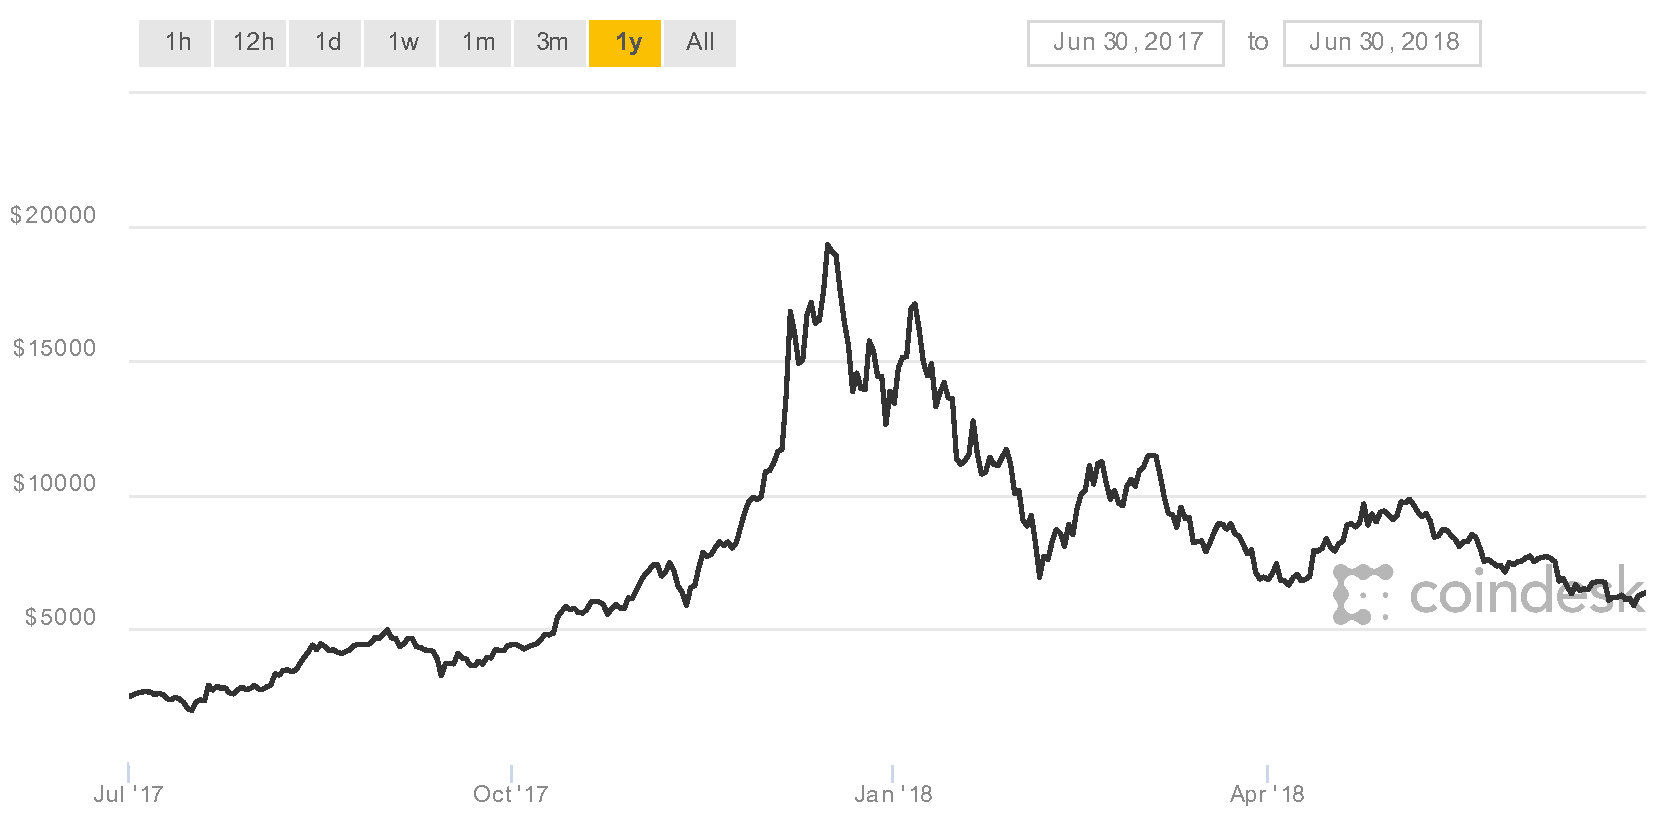
\includegraphics[width=1\textwidth]{figures/coindesk-bpi-chart}
\end{figure}
\let\thefootnote\relax\footnotetext{\tiny{* Plot from Coindesk.com}}
\end{frame}

\begin{frame}{}
\begin{itemize}
\item 
\end{itemize}
\end{frame}

\vspace{\stretch{0.5}}

\begin{block}{}
\end{block}


}

\end{document}


